\PassOptionsToPackage{ELEC}{aaltologo}
\documentclass[logo=bluequo,normaltitle]{aaltoslides}
%\documentclass{aaltoslides} % DEFAULT
%\documentclass[first=purple,second=lgreen,logo=bquo,normaltitle,nofoot]{aaltoslides} % SOME OPTION EXAMPLES

\usepackage[utf8]{inputenc}
\usepackage[T1]{fontenc}
\usepackage{graphicx}
\usepackage{amssymb,amsmath}
\usepackage{url}
\usepackage{lastpage}
\usepackage{epstopdf}
%\usepackage[pdfpagemode=None,colorlinks=true,urlcolor=red, linkcolor=black,citecolor=black,pdfstartview=FitH]{hyperref}
\usepackage{mdframed}
\usepackage{caption}
\usepackage{apacite}
\usepackage{listings}
\usepackage{adjustbox}
\usepackage[nomessages]{fp}

\usepackage{tikz}
\usetikzlibrary{positioning,shapes,shadows,arrows}
\tikzset{
  every overlay node/.style={
    %draw=black,fill=white,rounded corners,
    anchor=north west, inner sep=0pt,
  },
  thick/.style=      {line width=0.3mm},
}
\def\tikzoverlay{
   \tikz[remember picture, overlay]\node[every overlay node]
}%


%%%%%%%%%%%%%%%The functions are collected here %%%%%%%%%%%%%%%%%%%%%%%%%%%%%%%%%%%%%%%
%Intermediate section title slide
\newcommand{\slaikka}[1][Sectiontitle]{
    \section{#1}
    \begin{frame}[c]
    	\frametitle{}
        \begin{center}
            {\Large \color{primarycolor}{\textbf{#1}}}
        \end{center}
    \end{frame}
}

%%%% This for easy placemnet of figure inside a block
\newcommand{\putfig}[3][1.0]{
    \begin{block}{#3}
        \includegraphics[width=#1\linewidth,height=#1\textheight,keepaspectratio]{#2}
    \end{block}
}

%This is for a box 
\newcommand{\tbox}[3][0.3]{
    \tikzoverlay (n1) at (#2) {%
        \begin{tikzpicture}[every node/.style={inner sep=0.5ex,outer sep=0}]
            \tikzstyle{item}=[rectangle, draw=black, rounded corners, 
                    fill=secondarycolor!10, drop shadow,
                    text centered, anchor=north, text=black] 
                    \node (thenode)[item, rectangle]{
                        \begin{minipage}{#1\linewidth} #3 \end{minipage}};
        \end{tikzpicture}
    };
}
%%%%%%%%%%%%%%%%%%%%%%%%%%%%%%%%%%%%%%%%%%%%%%%%%%%%%%%%%%%%%%%%%%%%%%%%%%%%%%
%This is for a image. For titled image, use putfig 
\newcommand{\timage}[3][0.3]{
    \tikzoverlay (n1) at (#2) {%
        \begin{tikzpicture}[every node/.style={inner sep=0.5ex,outer sep=0}]
            \tikzstyle{item}=[rectangle, draw=black, rounded corners, 
                    fill=secondarycolor!10, drop shadow,
                    text centered, anchor=north, text=white] 
                    \node (thenode)[item, rectangle]{
                        \includegraphics[width=#1\textwidth,height=#1\textheight,keepaspectratio]{#3}};
        \end{tikzpicture}
    };
}


%Ellipse
\newcommand{\tellipse}[4]{
    \begin{tikzpicture}[overlay]
        \draw[secondarycolor,thick] (#1,#2) ellipse (#3 and #4);
    \end{tikzpicture}
}

%Arrow
\newcommand{\tarrow}[2]{
    \begin{tikzpicture}[overlay]
        \draw[secondarycolor,thick,->] (#1) -- (#2);
    \end{tikzpicture}
}


%%%% To insert lecture date
%\newcommand{\lectdate}{19.11.2015}
\newcommand{\lectdate}{\today}
\newcommand{\slidetitle}{TheSyDeKick tutorial}
%%%%

\title{\slidetitle}

\author[Marko Kosunen]{Marko Kosunen}
\institute[MNT]{Department of Micro and Nanosciences\\
Aalto University, School of Electrical Engineering\\marko.kosunen@aalto.fi}

\aaltofootertext{Analog macro releases}{\lectdate}{\arabic{page}/\pageref{LastPage}\ }

\date{\lectdate}


\begin{document}

\lstset{language=python,
    basicstyle=\small,
    stringstyle=\ttfamily
} 

\newcommand{\setlines}[2][1]{
    \FPeval{\firstline}{clip(#1)}
    \FPeval{\lines}{clip(#2)}
    \FPeval{\lastline}{clip(\firstline+\lines-1)}
}
\newcommand{\nextlines}[1][\lines]{
    \FPeval{\firstline}{clip(\lastline+1)}
    \FPeval{\lines}{clip(#1)}
    \FPeval{\lastline}{clip(\firstline+\lines-1)}
}

\newcommand{\codeclip}[2][python]{
    \FPeval{\scale}{min(clip(0.44/25*\lines),0.44)}
    \begin{adjustbox}{height=\scale\textheight , keepaspectratio}
    \lstinputlisting[
        frame=L, 
        numbers=left, 
        showlines=true
        language=#1, 
        firstline=\firstline, 
        lastline=\lastline, 
        firstnumber=\firstline]{#2}
    \end{adjustbox}
}
\newcommand{\setol}[1][0]{
    \FPeval{\oln}{clip(#1)}
}
\newcommand{\incol}{
    \FPeval{\oln}{clip(\oln+1)}
}

%%%%%%%%%%%%%%%%%%%%%%%%%%%%%%%%%%%%%%%%%%%%%%%%%%%%%%%%%%%%%%%%%%%%%%%%%%%%%%%%%%%%%%%%%%%%%
% Generates the titleframe
\aaltotitleframe
%%%%%%%%%%%%%%%%%%%%%%%%%%%%%%%%%%%%%%%%%%%%%%%%%%%%%%%%%%%%%%%%%%%%%%%%%%%%%%%%%%%%%%%%%%%%%

%%%%%%%%%%%%%%%%%%%%%%%%%%%%%%%%%%%%%%%%%%
%%%% CONTENTS %%%%%%%%%%%%%%%%%%%%%%%%%%%%
%%%%%%%%%%%%%%%%%%%%%%%%%%%%%%%%%%%%%%%%%%
\renewcommand{\sectionname}{Outline}
\section*{\sectionname}
\begin{frame}[c]
    \frametitle{\sectionname}
    \tableofcontents
\end{frame}

%%%%%%%%%%%%%%%%%%%%%%%%%%%%%%%%%%%%%%%%%%%
\begin{frame}[t]
    \frametitle{Prerequisites}
    \begin{itemize}
        \item Project template is available at
            \emph{https://github.com/TheSystemDevelopmentKit/thesdk\_template}.
        \item Alternatively you should have access to your project's
            TheSyDeKick repository at \emph{https://bubba.ecdl.hut-fi:81}
            \item You MUST have ssh keys set up for GitHub and ECD GitLab at
                bubba.
    \end{itemize}
\end{frame}

%%%%%%%%%%%%%%%%%%%%%%%%%%%%%%%%%%%%%%%%%%%%%%%%%%%%%%%%%%%%%%%%%%%%%%%%%%%%%%%%%%%%%%%%%%%%%
\sectiontitle[TheSyDeKick project structure]


%%%%%%%%%%%%%%%%%%%%%%%%%%%%%%%%%%%%%%%%%%%
\begin{frame}[t,fragile]
    \frametitle{Directory structures of TheSyDeKick project}
    \begin{itemize}
            \item All TheSyDeKick projects look the same
        \end{itemize}
    \adjustbox{height=0.4\textheight}{%
\begin{lstlisting}
TheSyDeKick_project
    init_submodules.sh     
    configure              
    sourceme.csh           
    pip3userinstall.sh   
    Entities                  <- All design modules are ``entities''
        thesdk                <- The SyDeKick core entity
        rtl                   <- rtl entity for rtl simulations
        spice                 <- spice entity for analog simulations
        thesdk_helpers
            shell
                initentity.sh <- Shell script for creating new entities
        inverter_tests
        inverter_testbench
        inverter              <- Example entity inverter. All entities look the same
            init_submodules.sh
            configure
            doc
            sv
            spice
            vhdl
            simulations      <- Temporary directory for simulation results
                rtlsim
            inverter
                __init__.py   <- Python description of the entity
                controller.py <- Additional entity related Python
\end{lstlisting}
}
\end{frame}


%%%%%%%%%%%%%%%%%%%%%%%%%%%%%%%%%%%%%%%%%%%
\begin{frame}[t,fragile]
    \frametitle{TheSyDeKick project structure} 
    \begin{itemize}
            \item All TheSyDeKick projects look the same
            \item TheSydeKick entities are git submodules initiated in the
                \emph{init\_submodules.sh}
            \item TheSydeKick entitities are transferable to any
                TheSyDeKick project.
            \item TheSydeKick entities are transferable to any
                TheSyDeKick project.
            \item TheSydeKick entities do not run stand-alone. They need the
                project.
            \item Obey the structure. It is not yours to change.
            \item New entities are initiated with
                \emph{thesdk\_helpers/shell/initentity.sh}
        \end{itemize}
\end{frame}

%%%%%%%%%%%%%%%%%%%%%%%%%%%%%%%%%%%%%%%%%%%
\sectiontitle[Testing the environment]

%%%%%%%%%%%%%%%%%%%%%%%%%%%%%%%%%%%%%%%%%%%
\begin{frame}[t,fragile]
    \frametitle{Testing the environment} 
    \begin{itemize}
            \item To test TheSyDeKick installation, do the following
        \end{itemize}
%    \adjustbox{height=0.4\textheight}
\begin{itemize}
    \item The, \textbf{check the Python versions from Thesdk.config} file. Version 3.6 is OK
        for ECD computing machines.
    \item Thesdk.config is created and will be overwritten by the configure
        script. Usually no need to re-run it. 
\end{itemize}

\end{frame}

%%%%%%%%%%%%%%%%%%%%%%%%%%%%%%%%%%%%%%%%%%%
\begin{frame}[t,fragile]
    \frametitle{Testing the environment} 
    \begin{itemize}
            \item Then we test the simulation execution
        \end{itemize}
%    \adjustbox{height=0.4\textheight}
\begin{itemize}
    \item Simulation of an inverter modeled in Python, verilog, vhdl and eldo
        is executed. 
    \item Press \emph{Return} to close the figures
    \item This is the elementary way of running simulations
    \item The ''production way'' is 
\end{itemize}
\begin{lstlisting}
./configure  && make sim          
\end{lstlisting}
\begin{itemize}
    \item Try it. If it works, you are good to go for the next step.
\end{itemize}
\end{frame}
%%%%%%%%%%%%%%%%%%%%%%%%%%%%%%%%%%%%%%%%%%%
\sectiontitle[Creating a new Entity]

%%%%%%%%%%%%%%%%%%%%%%%%%%%%%%%%%%%%%%%%%%%
\begin{frame}[t,fragile]
    \frametitle{Creating a new Entity} 
    \begin{itemize}
        \item All the Entities are eventually git submodules.
        \item Go through the following steps and try to think what happens in
            in term of version control
        \item The <my\_entity> refers to the entity you are creating. \emph{it should be
            replaced with your entity name}
        \item By default, the remote points to GitHub, and you do not have
            push permissions there.
        \end{itemize}
\adjustbox{height=0.21\textheight}{%
\begin{lstlisting}
cd entities
./thesdk_helpers/shell/initentity -h
./thesdk_helpers/shell/initentity <my_entity>
cd Entities/<my_entity>
#This is just to test the operation 
python3 <my_entity>/__init__.py  
git remote -v
git remote remove origin
git remote add origin \
    <URL of your TheSyDeKickgroup/<my_entity>.git 
git push --set-upstream origin master 
\end{lstlisting}
}
\end{frame}

%%%%%%%%%%%%%%%%%%%%%%%%%%%%%%%%%%%%%%%%%%%
\begin{frame}[t,fragile]
    \frametitle{Converting the new entity to submodule} 
    \begin{itemize}
        \item Go through the following steps and try to think what happens in
            in term of git submodules
    \end{itemize}
%    \adjustbox{height=0.4\textheight}
\end{frame}

%%%%%%%%%%%%%%%%%%%%%%%%%%%%%%%%%%%%%%%%%%%
\begin{frame}[t,fragile]
    \frametitle{Working with the submodules} 
    \begin{itemize}
        \item If you want to edit a submodule \emph{within the master project}
                this is how it goes
    \end{itemize}
%    \adjustbox{height=0.4\textheight}
\end{frame}
%%%%%%%%%%%%%%%%%%%%%%%%%%%%%%%%%%%%%%%%%%%
\sectiontitle[Simplifying the model to the bone]

%%%%%%%%%%%%%%%%%%%%%%%%%%%%%%%%%%%%%%%%%%%
\begin{frame}[t,fragile]
    \frametitle{The most simple  TheSyDeKick model} 
    \begin{itemize}
        \item The template (<my\_entity>) contains features that support
            python,eldo and rtl simulations.
        \item Next, we will remove all the parts from the model, and leave
            only the python model in place.
    \end{itemize}
\end{frame}

%%%%%%%%%%%%%%%%%%%%%%%%%%%%%%%%%%%%%%%%%%%
\begin{frame}[t,fragile]
    \frametitle{The target code} 
\end{frame}

%%%%%%%%%%%%%%%%%%%%%%%%%%%%%%%%%%%%%%%%%%%
\setlines{21}
\begin{frame}[t,fragile]
    \frametitle{The target code} 
    \begin{itemize}
        \item Edit the \emph{Docstring}
    \end{itemize}
    \codeclip{./thesdk_template/Entities/myentity/myentity/__init__.py}
\end{frame}

%%%%%%%%%%%%%%%%%%%%%%%%%%%%%%%%%%%%%%%%%%%
\nextlines[8]
\begin{frame}[t,fragile]
    \frametitle{The target code} 
    \begin{itemize}
        \item Edit the \emph{package imports}
    \end{itemize}
    \codeclip{./thesdk_template/Entities/myentity/myentity/__init__.py}
\end{frame}

%%%%%%%%%%%%%%%%%%%%%%%%%%%%%%%%%%%%%%%%%%%
\nextlines[52]
\begin{frame}[t,fragile]
    \frametitle{The target code} 
    \begin{itemize}
        \item Edit the \emph{Class definition}
    \end{itemize}
    \codeclip{./thesdk_template/Entities/myentity/myentity/__init__.py}
\end{frame}

%%%%%%%%%%%%%%%%%%%%%%%%%%%%%%%%%%%%%%%%%%%
\nextlines[45]
\begin{frame}[t,fragile]
    \frametitle{The target code} 
    \begin{itemize}
        \item Edit the \emph{Main script}
    \end{itemize}
    \codeclip{./thesdk_template/Entities/myentity/myentity/__init__.py}
\end{frame}

%%%%%%%%%%%%%%%%%%%%%%%%%%%%%%%%%%%%%%%%%%%
\nextlines[45]
\begin{frame}[t,fragile]
    \frametitle{The target code} 
    \begin{itemize}
        \item Now you are ready to run you model
    \end{itemize}
\begin{lstlisting}
cd Entities/<my_entity>
#This is just to test operation 
python3 <my_entity>/__init__.py  
\end{lstlisting}
    \begin{itemize}
        \item The result should look like this:
    \end{itemize}
    \begin{center}
        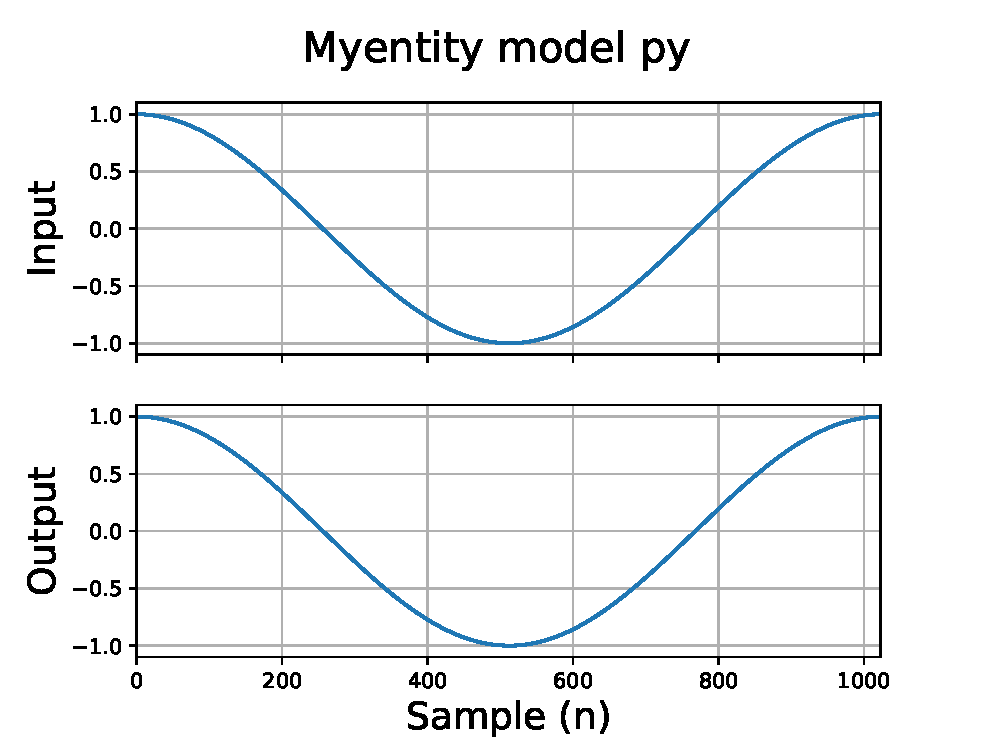
\includegraphics[width=0.6\textwidth]{./thesdk_template/Entities/myentity/myentity/inv_py.eps}
    \end{center}
\end{frame}

%%%%%%%%%%%%%%%%%%%%%%%%%%%%%%%%%%%%%%%%%%%
\nextlines[45]
\begin{frame}[t,fragile]
    \frametitle{Running with make } 
    \begin{itemize}
        \item You can now try to run the test with the ``Production method''
    \end{itemize}
\begin{lstlisting}
#cd Entities/<my_entity>
./configure
make sim
\end{lstlisting}
    \begin{itemize}
        \item The result should be the same:
    \end{itemize}
    \begin{center}
        %This is generated by make
        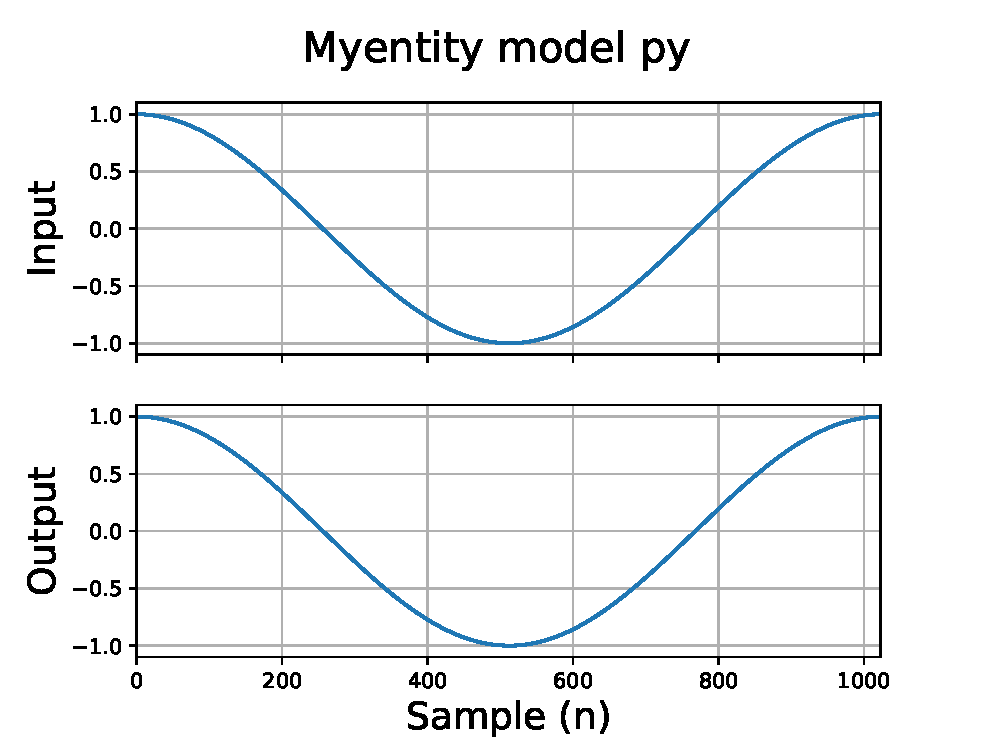
\includegraphics[width=0.6\textwidth]{./thesdk_template/Entities/myentity/myentity/inv_py.eps}
    \end{center}
\end{frame}

%%%%%%%%%%%%%%%%%%%%%%%%%%%%%%%%%%%%%%%%%%%
\sectiontitle[Documentation with Doctrings]

%%%%%%%%%%%%%%%%%%%%%%%%%%%%%%%%%%%%%%%%%%%
\begin{frame}[t,fragile]
    \frametitle{Building the documentation} 
    \begin{itemize}
        \item TheSyDeKick takes also care for you basic documentation needs
        \item We are ysing Python Docstrings for that. You may do a web search
            to figure out what it means.
        \item Create the documentation or your module with:

    \end{itemize}
\begin{lstlisting}
#cd Entities/<my_entity>
./configure
make doc
\end{lstlisting}
\end{frame}

%%%%%%%%%%%%%%%%%%%%%%%%%%%%%%%%%%%%%%%%%%%
\begin{frame}[t,fragile]
    \frametitle{Reading the documentation} 
    \begin{itemize}
        \item You may read the documentation with
    \end{itemize}
\begin{lstlisting}
#cd Entities/<my_entity>
firefox ./doc/build/html/index.html
\end{lstlisting}
    \begin{itemize}
        \item Compare the documentation to your source code. You may already
            guess how it is created.
    \end{itemize}
    \begin{center}
        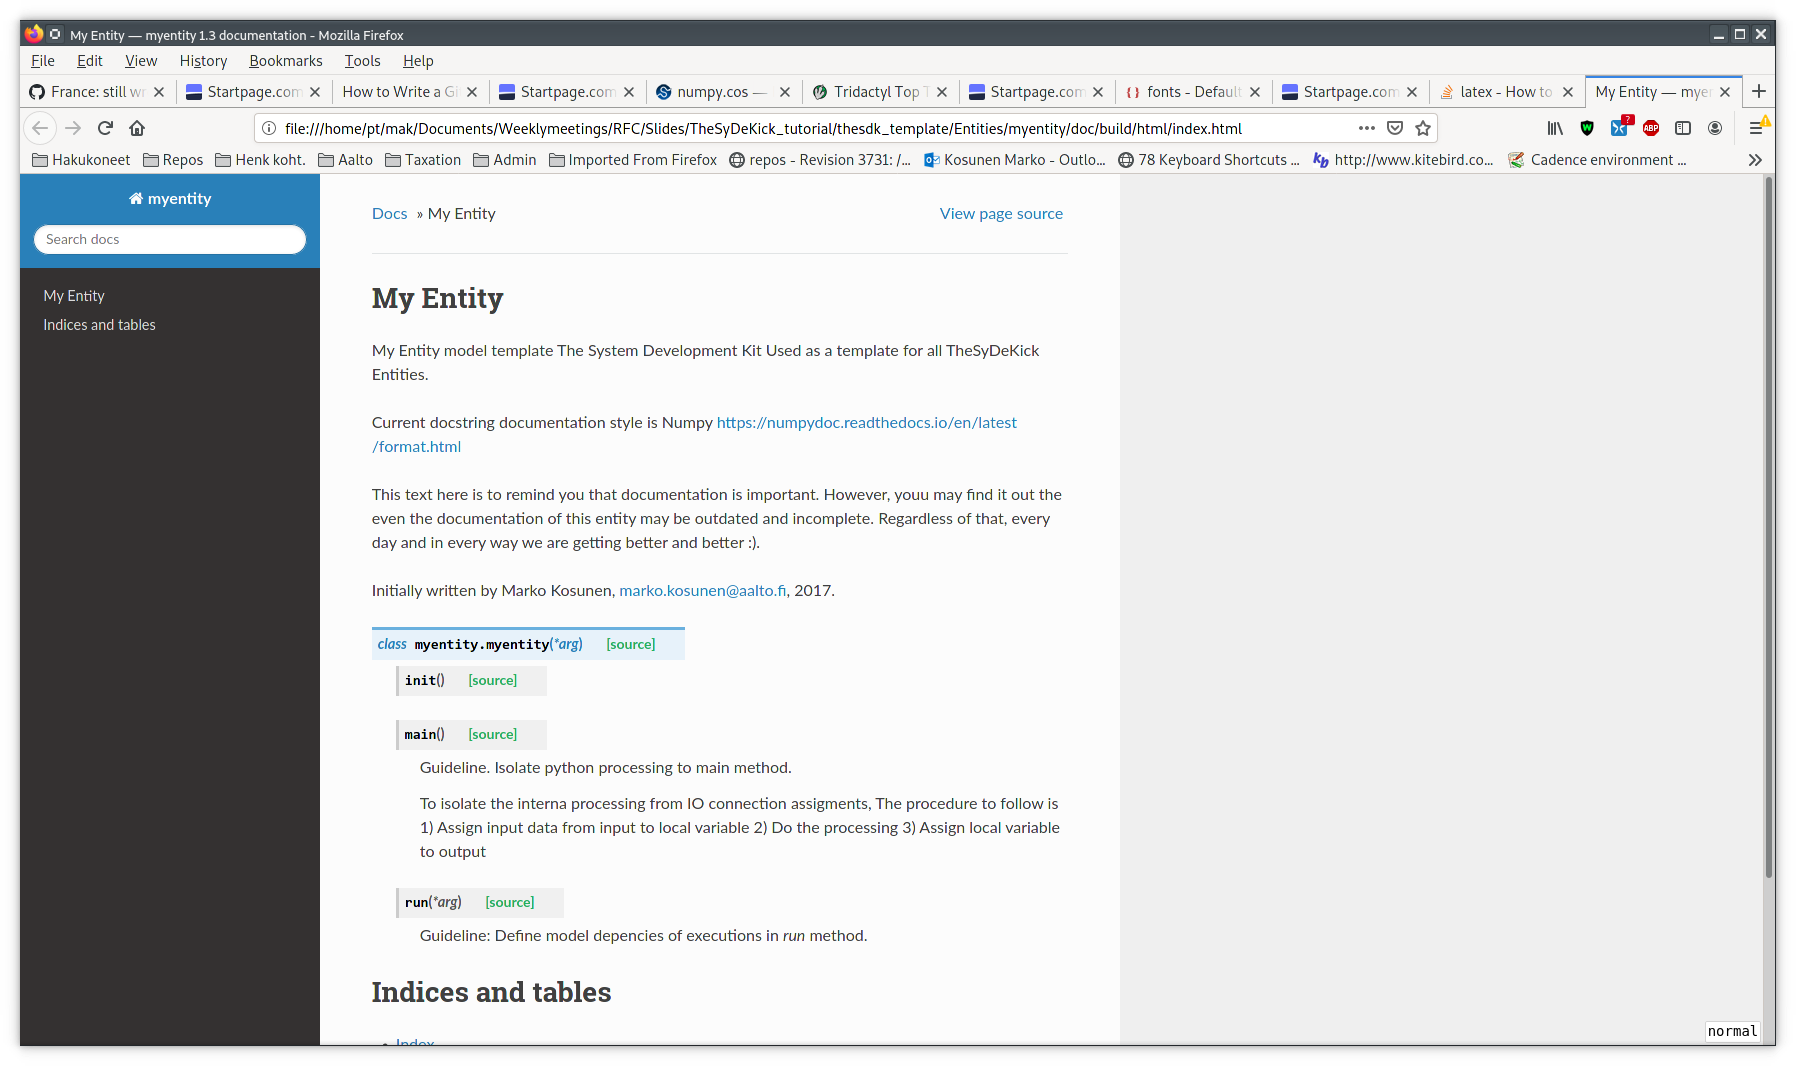
\includegraphics[width=0.7\textwidth]{./Pics/Documentation.png}
    \end{center}
\end{frame}

%%%%%%%%%%%%%%%%%%%%%%%%%%%%%%%%%%%%%%%%%%%
\sectiontitle[Getting production ready]

%%%%%%%%%%%%%%%%%%%%%%%%%%%%%%%%%%%%%%%%%%%
\begin{frame}[t,fragile]
    \frametitle{Production version } 
    \begin{itemize}
        \item To minimize the need for documentation, TheSydeKick follows the
            following principles
            \begin{itemize}
                \item \emph{./init\_submodules.sh} gets the submodules
                \item \emph{configure} does the configuration and creates the
                    Makefile
                \item \emph{make} does the actual work with some functional
                    defaults, and creates the documentation.
            \end{itemize}
        \item You should be now ready to build you module as it is in
            production.
    \end{itemize}
\begin{lstlisting}
#cd Entities/<my_entity>
configure && make
\end{lstlisting}
    \begin{itemize}
        \item Press \emph{Return} close the figure.
        \item This runs the simulation and generates the documentation. 
        \item You may study the structure of \emph{configure}
        \item You are now ready to release your module:
    \end{itemize}
\begin{lstlisting}
git add -i  #Select the files you have edited
git commit `# Give a nice and clean commit message
git push    
\end{lstlisting}
\end{frame}

%%%%%%%%%%%%%%%%%%%%%%%%%%%%%%%%%%%%%%%%%%%
\begin{frame}[t,fragile]
    \frametitle{Working with the submodules, again} 
    \begin{itemize}
        \item As you are workin \emph{within the master project}
                remember to update it
    \end{itemize}
%    \adjustbox{height=0.4\textheight}
\end{frame}

%%%%%%%%%%%%%%%%%%%%%%%%%%%%%%%%%%%%%%%%%%%
\sectiontitle[Congratulations, You are DONE!]

\end{document}
